\chapter{Materials and Methods}

\section{Dataset Description}
Two experimental datasets were available.
In the first study, 59 acute comatose patients were included between 7 days and 30 days after coma onset (46 ± 16 years old; 21 females).
PET data were acquired in list mode for 90 minutes following an intravenous bolus injection of \fdg.
The second study included 7 healthy subjects (25 ± 3 years old; all male) who received an intravenous bolus of \yohimbine.

Both datasets used the same imaging protocol.
Using a Siemens Healthineers Biograph mMR simultaneous MR–PET system, an arterial time-of-flight MR angiography (TOF-MRA) was acquired in axial orientation with a voxel size of 0.3\(\times\)0.3\(\times\)0.7 mm, and a T1-weighted MRI was acquired in axial orientation with isotropic 1 mm voxels, during the 90-minute dynamic PET.
Raw PET data were rebinned into 24 time frames (variable-length frames: 8\(\times\)15 s, 3\(\times\)60 s, 5\(\times\)120 s, 1\(\times\)300 s, 7\(\times\)600 s) sinograms for dynamic reconstruction.
Reconstruction yielded a voxel size of 1.04\(\times\)1.04\(\times\)2.08 mm\(^3\) in a matrix of 344\(\times\)344\(\times\)127 voxels.

In the \fdg\ study, whole-blood and plasma AIFs were measured from 26 manually collected arterial samples (timing: every 5 s for the first minute, every 15 s until the second minute, and at 3, 5, 10, 20, 30, 45, 60, 75, 80, 85, and 90 minutes post-injection) and counted in a gamma counter.
In the \yohimbine\ study, 25 arterial blood samples were manually collected (timing: every 5 s for the first minute, every 10 s until the second minute, and at 5, 10, 30, 45, 60, and 90 minutes post-injection).
The blood samples were counted in a gamma counter, then centrifuged to separate plasma, and the plasma activity was measured to compute the plasma fraction as the ratio of plasma to whole-blood activity at each time point.

\section{Pre-processing}
For both studies, the T1-weighted image was registered to the average PET image and to the TOF-MRA using the NiftyReg program, an affine registration method \cite{modat2014global}.
The two resulting affine transformation matrices were then composed to register the TOF-MRA directly to the PET space.
Even though patients in the \fdg\ study were unconscious and PET and MRI were acquired simultaneously in the same session, we performed this step out of caution to eliminate the possibility of misregistration.
The T1-weighted image served as an intermediary because it shares anatomical features with both modalities, whereas directly registering TOF-MRA to PET is impractical due to PET’s lower spatial resolution and the limited axial field-of-view of TOF-MRA.
Finally, the brain in the T1-weighted image was segmented into regions of interest (ROIs) using the Hammersmith brain atlas \cite{hammers2003three} to obtain regional masks, and these masks were applied to the dynamic PET to extract regional TACs.


\section{Carotid Segmentation\label{sec:carotid}}
Figure~\ref{fig:seg_pipeline} summarizes the carotid segmentation pipeline.
Because vessels appear hyperintense in TOF-MRA, a high-intensity threshold can extract arterial structures.
However, lesions—which were common in the comatose cohort—and venous structures can also appear hyperintense, and may be inadvertently selected by thresholding.
To exclude these, a cuboid volume of interest (VOI) was defined in a reference space to cover the anatomical region where the ICAs are most likely to appear (Step I).
The threshold was set to the 1st percentile of all non-zero voxels in the image and applied only within the VOI (Step II).
A 3D connected-components filter was then applied, and the two largest connected components were retained as the left and right internal carotid arteries (Step III).

The reference image was the standard MNI152 atlas, padded by 50\% in the inferior direction (negative \(z\) in voxel space) because the original atlas excludes the subcranial region relevant for the ICAs.
The TOF-MRA was registered to this reference using an affine transformation, and the resulting matrix was used to map the VOI into TOF-MRA space before applying the thresholding and connectivity steps.

\begin{figure}[h]
	\centering
	\begin{tikzpicture}[
			node distance=1cm,
			auto,
			>=Stealth,
			mybox/.style={draw, rounded corners, rectangle, minimum width=3cm, minimum height=1cm, align=center}
		]
		\node[mybox] (input) {TOF-MRA};
		\node[mybox, right=of input] (cuboid) {I) Cuboid Mask\\Application};

		\node[mybox, right=of cuboid] (thresh) {II) Adaptive\\ Threshold};
		\node[mybox, below=of thresh] (growing) {III) Largest 2 Regions};
		\node[mybox, left=of growing] (dilation) {IV) Dilation};
		\node[mybox, below=of growing] (mask) {Carotid\\Mask};
		\node[mybox, below=of dilation] (bg_mask) {Background\\Mask};

		\draw[->] (input) -- (cuboid);
		\draw[->] (cuboid) -- (thresh);
		\draw[->] (thresh) -- (growing);
		\draw[->] (growing) -- (mask);
		\draw[->] (growing) -- (dilation);
		\draw[->] (dilation) -- (bg_mask);
	\end{tikzpicture}
	\caption{Carotid and background mask segmentation pipeline}
	\label{fig:seg_pipeline}
\end{figure}

\section{Partial Volume Correction}

\subsection{Geometric Transfer Matrix}
As discussed before in Section~\ref{sec:pve}, direct extraction of the radioactivity in the arteries is not practical due to PVC.
Geometric Transfer Matrix aims to account for this loss of signal by considering the observed TACs are a linear combination of the true value and other affecting regions \cite{rousset1998correction}.

Here we define two regions, the carotid and the surrounding tissues (background).
A mask for extracting the activities of the latter was obtained by dilating the carotid mask by 5 mm and subtracting the voxels corresponding to the carotid mask (Figure~\ref{fig:seg_pipeline}, Step IV).

\begin{equation}
	\underbrace{
		\begin{bmatrix}
			T_{c} \\
			T_{bg}
		\end{bmatrix}
	}_{\text{Observed}}
	=
	\underbrace{
		\begin{bmatrix}
			\omega_{c \rightarrow c}  & \omega_{bg \rightarrow c}  \\
			\omega_{c \rightarrow bg} & \omega_{bg \rightarrow bg}
		\end{bmatrix}
	}_{\text{GTM}}
	.
	\underbrace{
		\begin{bmatrix}
			T_{IF} \\
			T_{tissue}
		\end{bmatrix}
	}_{\text{Unknown}},
\end{equation}
where $\omega_{n \rightarrow m}$ are the spill-in and spill-over coefficients of region $n$ onto region $m$, as defined below.
where
\begin{equation}
	\omega_{n\to m} = \frac{\displaystyle \int_{\Omega_m} \bigl( h \ast \chi_n \bigr)(r)\,dr}{\displaystyle \int_{\Omega_m} \bigl( h \ast \chi_m \bigr)(r)\,dr},
\end{equation}
with \(\chi_n\) and \(\chi_m\) denoting the binary masks of regions \(n\) and \(m\), respectively, \(h\) the system's point spread function, and \(\Omega_m\) the spatial domain of region \(m\).

$T_{c}$ and $T_{bg}$ are respectively the observed carotid and background TACs and $T_{IF}$ and $T_{tissue}$ are the real unknown TACs of the carotid (the input function) and the background tissue.

By inverting the GTM, this system of equations can be solved to recover the arterial and background TACs.
However, GTM and other classical PVC methods often fail to fully recover the lost signal because they simplify the problem and ignore time-varying noise characteristics.
As a result, they may propagate or even amplify noise.
Time-varying noise arises from several factors, including the small diameter of the ICAs, very short early frames when the IF changes rapidly, and the exponential decay of the tracer, all of which reduce gamma counts detection by the PET camera and increase variance.

\subsection{Bayesian Geometric Transfer Matrix}

\subsubsection{Modelling}\label{sec:bgtm_modelling}
For each subject, \(T_{IF}\) is modeled as a linear combination of a population mean and principal components obtained by applying principal component analysis (PCA) to AIFs from the cohort.
Specifically, for each subject, a subset of randomly selected subjects—excluding the subject under study—is used to build a PCA basis.
After zero-centering the training AIFs, PCA yields principal axes \(\phi_i(t)\) with explained variances \(\lambda_i\).
We define scaled components \(v_i(t) = \sqrt{\lambda_i}\,\phi_i(t)\), and write
\begin{equation}
	T_{IF}(t) = \mu_{IF}(t) + \sum_{i=1}^p \theta_i\,v_i(t),
\end{equation}
where \(\mu_{IF}(t)\) is the population mean and the coefficients satisfy \(\theta_i \sim \mathcal{N}(0,1)\) by construction.
Here, \(p\) denotes the number of retained components.

Spectral analysis (SA) models tissue activity as the convolution of the input function with an impulse response written as a sum of exponentials \cite{cunningham1993spectral}.
This makes it more flexible and generalizable as it does not assume a particular compartment model and is convenient for describing background signal.
Therefore, the background TAC is

\begin{equation}
	T_{bg}(t) = \sum_{i=1}^s \alpha_{i} \,\bigl(T_{IF} \circledast e^{-\beta_{i} t}\bigr)(t),
\end{equation}
where \(\circledast\) denotes convolution, \(\alpha_i\) is the amplitude, and \(\beta_i\) is the decay rate of the \(i\)th spectral component.

\subsubsection{Noise}
Accurate noise modeling is challenging because multiple sources contribute to the variance.
Some effects (e.g., scatter, randoms, and motion) are partially corrected during reconstruction post-processing.
The main contributor is low-count statistics, an inherent limitation of PET due to detector performance and overall camera sensitivity, which is particularly problematic for IDIF because the ICAs are small, early frames are very short during the bolus passage, and radioactive decay reduces detected events, increasing variance across frames.

While raw PET counts are Poisson-distributed, post-reconstruction noise is typically approximated as Gaussian \cite{TODO}.
To account for time-varying noise, we use per-frame weights to normalize variance across frames:
\begin{equation}
	\omega_{i} = \frac{\Delta t_i}{c_i}\,\exp\!\left(-\frac{t_{i}\,\ln 2}{T_{1/2}}\right),
\end{equation}
where \(\Delta t_i\) is the frame duration, \(c_i\) is the net true counts for frame \(i\), and \(T_{1/2}\) is the tracer half-life.
Because \(c_i\) was unavailable, we substitute \(C_T(t_i)\), the total reconstructed activity concentration at the frame mid-time.

The time-varying noise level is summarized by a weighted average variance:
\begin{equation}
	\sigma^2 = \frac{1}{N} \sum_{i=1}^{N} \omega_i\,\sigma_i^2.
\end{equation}

\subsubsection{Estimation}
Let \(\mathcal{D}\) denote the observed PET TAC, and let \( \Theta = (\theta_{1}, \dots,\theta_{p}, \alpha_{1}, \beta_{1}, \dots, \alpha_{s}, \beta_{s}) \) be the unknown model parameters, with an unknown Gaussian noise variance \(\sigma^2\).
We aim to estimate the joint posterior \(p(\Theta,\sigma^2\mid \mathcal{D})\).

By Bayes’ rule,
\begin{equation}\label{eq:posterior}
	p(\Theta,\sigma^2 \mid \mathcal{D}) \propto p(\mathcal{D} \mid \Theta,\sigma^2)\,\pi( \Theta )\,\pi( \sigma^2),
\end{equation}
where \(p(\mathcal{D} \mid \Theta,\sigma^2)\) is the likelihood and \(\pi(\cdot)\) are the priors.
We can therefore sample the posterior once the likelihood and priors are obtained.

The observed data are linked to the latent TACs through GTM.
For convenience, define
\begin{equation}
	\mathcal{T}(t) = \mathcal{G}(t;\Theta) =
	\mathcal{G}\!\left(
	\begin{bmatrix}
			T_{IF}(t;\theta_{1}, \dots, \theta_{p}) \\
			T_{tissue}(t;\alpha_{1}, \beta_{1}, \dots)
		\end{bmatrix}\right),
\end{equation}
where \(\mathcal{G}\) is the GTM operator and \(\mathcal{T}\) is the predicted activity (after PVE).
Assuming Gaussian noise with frame weights \(\omega_i\), the likelihood is
\begin{equation}
	p(\mathcal{D} \mid \Theta,\sigma^2) = \prod_{i=1}^N \frac{1}{\sqrt{2\pi \sigma^2}} \exp\!\left( -\frac{\omega_i,\bigl(\mathcal{D}(t_i) - \mathcal{T}(t_i)\bigr)^2}{2\sigma^2} \right).
\end{equation}
We refer to this framework as the Bayesian Geometric Transfer Matrix (Bayesian GTM or BGTM).

The prior factorizes as
\begin{equation}
	\pi(\Theta) = \prod_{i=1}^p \pi(\theta_i)\,\prod_{j=1}^s \pi(\alpha_j)\,\pi(\beta_j).
\end{equation}
As noted above, \(\theta_i \sim \mathcal{N}(0,1)\).
For the spectral parameters, we adopt broad uniform priors,
\begin{equation}
	\alpha_i,\beta_i \sim \mathcal{U}( u_{\text{min}} , u_{\text{max}} ).
\end{equation}

For the noise variance, we use an inverse-gamma prior, \(\pi(\sigma^2) \sim \Gamma^{-1}(a_0,b_0)\), conjugate to the Gaussian likelihood.
We center this prior around an empirical weighted mean squared deviation between the observed carotid TAC and the mean AIF:
\begin{equation}
	\mathbb{E}[X] = \frac{1}{N} \sum_{i=1}^{N} \omega_i\,\bigl(T_c(t_i) - \mu_{IF}(t_i)\bigr)^2.
\end{equation}
Given a chosen coefficient of variation (CV), we set
\begin{equation}
	a_0 = 2 + \frac{1}{\mathrm{CV}^2}, \qquad b_0 = (a_0 - 1)\,\mathbb{E}[X].
\end{equation}

\subsubsection{Sampling}
Direct evaluation of the posterior in \eqref{eq:posterior} is intractable, so we employ Monte Carlo sampling.
We use a Markov chain Monte Carlo scheme with a Metropolis-within-Gibbs strategy.

Gibbs updates draw each parameter from its univariate conditional posterior \(p(\Theta_i \mid \mathcal{D}, \Theta_{-i}, \sigma^2)\) and the noise variance from \(p(\sigma^2 \mid \mathcal{D},\Theta)\).
Metropolis–Hastings proposals explore \(\Theta\): at iteration \(m\), propose \(\Theta_{i}^\prime = \Theta_{i}^{(m)} + \varepsilon_{i}\,b\), where \(\varepsilon_i\) is the step size and \(b\) is a Brownian perturbation.
Accept with probability
\begin{equation}
	\min\!\left(1,\ \frac{p(\Theta_i^\prime \mid \mathcal{D}, \Theta_{-i}, \sigma^2)}{p(\Theta_i^{(m)} \mid \mathcal{D}, \Theta_{-i}, \sigma^2)}\right).
\end{equation}

Because the inverse-gamma prior is conjugate, the conditional posterior for \(\sigma^2\) is also inverse-gamma,
\begin{equation}
	p(\sigma^2 \mid \mathcal{D},\Theta) \sim \Gamma^{-1}(a, b),
\end{equation}
with
\begin{equation}
	a = a_0 + \frac{N}{2}, \qquad b = b_0 + \frac{1}{2}\sum_{i=1}^{N} \omega_i\,\bigl(\mathcal{D}(t_i) - \mathcal{T}(t_i)\bigr)^2.
\end{equation}
Thus, \(\sigma^2\) can be sampled directly without Metropolis–Hastings.

To improve mixing, each parameter \(k\) has its own proposal step size \(\epsilon_k\).
During burn-in, step sizes are adapted every \(L=50\) Metropolis–Hastings updates by an arbitrary acceptance rate of 0.5: if the empirical rate exceeds 0.5, increase \(\epsilon_k \leftarrow 1.1\,\epsilon_k\); otherwise decrease \(\epsilon_k \leftarrow 0.9\,\epsilon_k\).
After burn-in, step sizes are fixed and subsequent samples are retained.

\subsubsection{Inference}
After sufficient sampling, we use a modified maximum a posteriori (MAP) estimate by averaging the parameters of the top 0.1\% of samples ranked by posterior probability and reporting this average as the solution.
\section{Plasma Fraction Correction}
By construction, IDIFs extracted from PET represent whole-blood activity.
For \fdg, plasma metabolites are generally negligible over the scan, so the whole-blood AIF was used without plasma or metabolite correction \cite{gambhir1989simple}.
For \yohimbine, kinetic modeling requires the plasma parent activity, so whole-blood IDIFs were converted to plasma and corrected for metabolites using
\begin{equation}
	C_{P,\mathrm{parent}}(t) \;=\; \frac{C_{WB,\mathrm{IDIF}}(t)}{R_{bp}} \,\times\, \mathrm{PPF}(t),
\end{equation}
where \(R_{bp}=0.661\) is the whole-blood–to–plasma ratio and \(\mathrm{PPF}(t)\) is the plasma parent fraction modeled as a three-exponential curve \cite{laurencin2021modeling}:
\begin{equation}
	\mathrm{PPF}(t) \;=\; 0.30\,e^{-t/0.88} \;+\; 0.09\,e^{-t/11.49} \;+\; 0.61\,e^{-t/65.77}.
\end{equation}
Because \(V_T\) estimation uses total plasma parent activity, no additional free-fraction correction was applied.

\section{Evaluation}

\subsection{IF Curves}
The performance of the proposed IDIF estimation was first evaluated by computing the mean absolute error (MAE) between the cumulative area under the curve (cAUC) of the estimated IDIF and the \textit{ground truth} AIF.
cAUC was considered to be a more suitable metric since it provides an integrated measure of tracer exposure over time and is less sensitive to local fluctuations or noise in the curve compared with directly comparing the TACs.
\begin{equation}
	\textrm{cAUC}(t) =  \int_{0}^{t} IF(\tau) \, d\tau,
\end{equation}
where \(IF\) is the input function.

\subsection{Quantification}
However, because the cAUC error does not fully capture the impact of IDIF deviations on kinetic parameters, absolute quantification was also performed to evaluate the performance of the estimated IDIF against the gold standard AIF.
Quantification was performed using graphical methods implemented in TPCCLIB \cite{oikonen2018tpcclib}.
The Patlak plot was used for \fdg\ \cite{patlak1983graphical}, and the Logan plot for \yohimbine\ \cite{logan1990graphical}.

The brain atlas was applied to the PET image and regional TACs were obtained by averaging voxels over time.
For \fdg, regional \(\mrglu\) was computed.
The mean absolute percentage error (MAPE) of \(\textrm{MR}_{\textrm{glu}}\) in each ROI was then calculated and averaged across the dataset:
\begin{equation}
	\text{Average MAPE}(\mrglu)= \frac{100}{N} \sum_{i=1}^{N} \left( \frac{1}{N_{\text{ROI}}} \sum_{j=1}^{N_{\text{ROI}}} \left| \frac{\textrm{MR}_{\textrm{glu},ij}^{\textrm{IDIF}} - \textrm{MR}_{\textrm{glu},ij}^{\textrm{AIF}}}{\textrm{MR}_{\textrm{glu},ij}^{\textrm{AIF}}} \right| \right),
\end{equation}
where \(N\) is the number of subjects.

Similarly, for \yohimbine, the volume of distribution (\(V_T\)) was calculated and the dataset error was computed as
\begin{equation}
	\text{Average MAPE}(V_T)
	= \frac{100}{N}
	\sum_{i=1}^{N}
	\biggl(
	\frac{1}{N_{\mathrm{ROI}}}
	\sum_{j=1}^{N_{\mathrm{ROI}}}
	\left|
	\frac{V_{T,ij}^{\mathrm{IDIF}} - V_{T,ij}^{\mathrm{AIF}}}
	{V_{T,ij}^{\mathrm{AIF}}}
	\right|
	\biggr).
\end{equation}

Additionally, linear least-squares regression was performed between the regional \(\mrglu\) and \(V_T\) obtained using AIF and IDIF for each subject.
The coefficient of determination (\(R^2\)) and regression slope (\(S\)) were computed per subject.
The mean absolute percentage errors of these metrics across the dataset are
\begin{equation}
	\text{Average MAPE}(R^2) = \frac{100}{N} \sum_{i=1}^{N} \left| R^2_i - 1 \right|
\end{equation}
and
\begin{equation}
	\text{Average MAPE}(S) = \frac{100}{N} \sum_{i=1}^{N} \left| S_i - 1 \right|,
\end{equation}
where \(R^2_i\) and \(S_i\) denote the coefficient of determination and slope for subject \(i\), respectively.

\section{Simulation}\label{sec:methods_simulation}
PET simulations are integral to validating statistical and analytical PET methods because they provide ground truth that may be unavailable or affected by human or instrumental error in experimental data.
In the previous section, we treated the AIF as the ground truth and evaluated methods against it.
However, because AIF measurement and analysis involve multiple manual steps and devices operated by different personnel, errors can occur.

Therefore, as a complementary validation, we conducted realistic simulations and evaluated the method on these data as well.
PET-SORTEO is a Monte Carlo PET simulation platform \cite{reilhac2004pet,reilhac2016validation} whose accuracy has been validated previously \cite{reilhac2005pet} and can closely approximate real acquisitions.
This fidelity strongly depends on accurate descriptions of both the physical anatomy and tracer kinetics.

As input, PET-SORTEO requires the description and geometry of the PET machine, a 3D emission phantom segmenting the tissues into emitting regions, a 3D attenuation phantom describing tissue attenuation coefficients, and TACs for each emitting region.
For this study, we simulated the \fdg\ dataset using the Biograph mMR model to mirror the experimental datasets, and we derived numerical phantoms and TACs from the real MR and PET data.
A schematic of the overall simulation pipeline is shown in Figure~\ref{fig:sim_pipeline}.

For each subject, first, the brain atlas subregions were merged into larger regions: white matter (WM), gray matter (GM), gray nuclei (GN), cerebellar gray matter (CGM), and cerebellar white matter (CWM).
An algorithm originally developed for pseudo-CT generation from T1-weighted MRI for bone attenuation correction was used to create masks for the extracerebral regions\cite{mérid2017}.
Values above 300 were labeled as bone (BONE) and values between \(-300\) and \(300\) after excluding the brain as extracerebral soft tissues (SOFT), which include the scalp, neck muscles, glands, and eyes.
The leftover space between the skull and the brain was labeled as cerebrospinal fluid (CSF).
Finally, the arterial mask (ICA) was obtained from the TOF-MRA segmentation (Section~\ref{sec:carotid}).
These nine regions were combined to form the emission phantom.

The attenuation phantom was generated from the pseudo-CT by segmenting SOFT and BONE and assigning their respective attenuation coefficients.

The emission phantom was then registered to PET space to extract subject-specific TACs.
These TACs were corrected for PVE using GTM and subsequently fitted with a 2TCM to denoise and obtain "ideal" TACs.
The AIF used for fitting was the subject’s measured AIF, itself fitted to an exponential model to remove noise \cite{feng1993models}.

Several practical considerations were applied.
Our SOFT definition is broad; while adequate for simulation, it violates homogeneity assumptions in compartment modeling, so the unfitted TAC was retained for SOFT.
The pseudo-CT algorithm was permissive for BONE, leading to overestimated BONE TACs due to spill-in; empirically, BONE activity was scaled by 0.5.

Extracting the correct activity of the CSF with this approach is not feasible since it's a very thin region which is heavily affected by PVE. Thus, CSF TAC was considered 0.2 of the fitted WM TAC.
\begin{figure}[h]
	\centering
	\begin{tikzpicture}[
			node distance=1cm and 2cm,
			auto,
			>=Stealth,
			mybox/.style={draw, rounded corners, rectangle, minimum width=2cm, minimum height=1cm, align=center}
		]

		\node[mybox,minimum width=3cm] (pet) {PET};
		\node[mybox,minimum width=3cm, below=of pet] (t1) {T1w MRI};
		\node[anchor=south east] at($(pet.north)+(0,0.5)$) (pet_image) {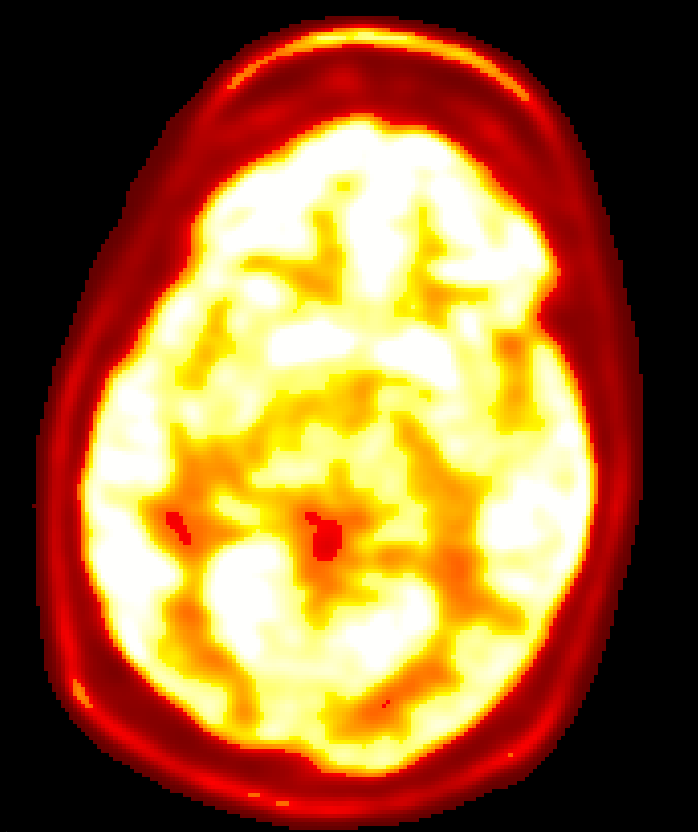
\includegraphics[height=3cm]{figures/real_pet.png}};
		\node[right=0.1cm of pet_image] (t1_image) {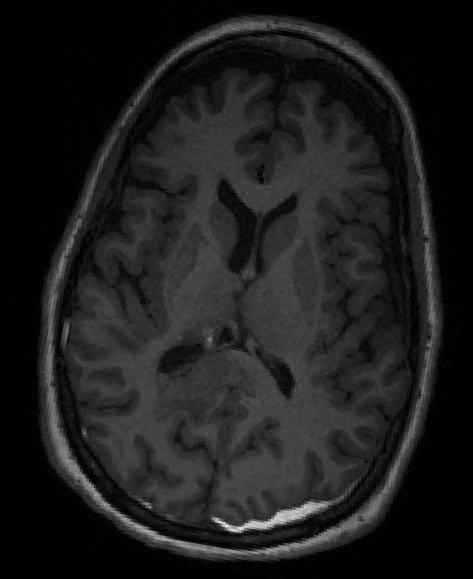
\includegraphics[height=3cm]{figures/t1.png}};


		\node[mybox, right=5cm of pet, minimum width=3cm] (ttac) {Tissue Activity};
		\node[mybox, right=5cm of t1, minimum width=3cm] (phantom) {Anatomical\\Phantom};

		\node[anchor=south east] at($(ttac.north)+(0,0.5)$) (phantom_image) {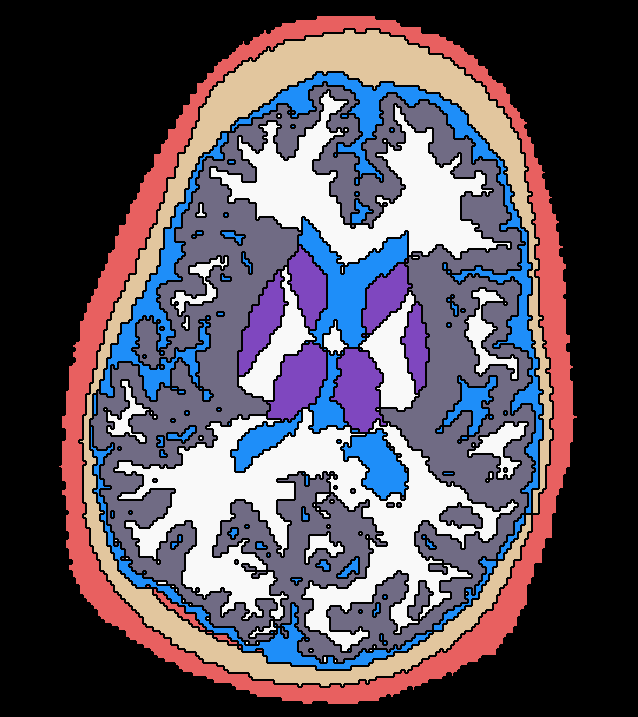
\includegraphics[height=3cm]{figures/phantom.png}};
		\node[right=0cm of phantom_image] (ttac_image) {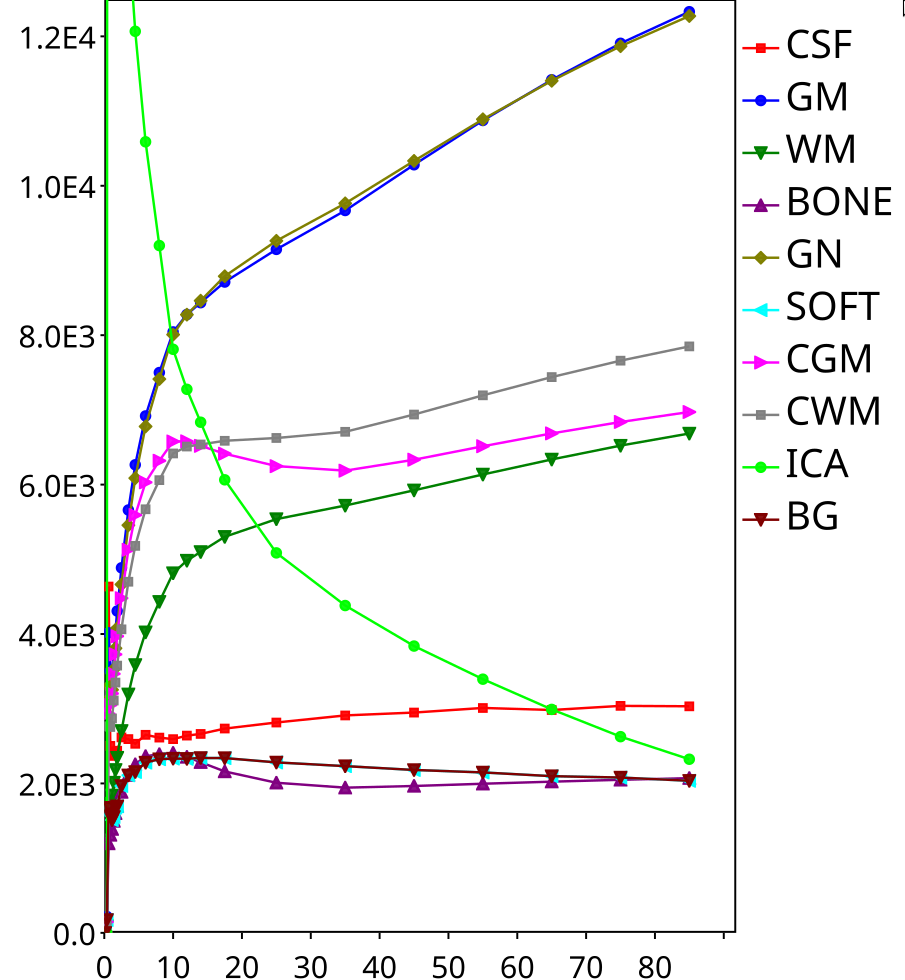
\includegraphics[height=2cm]{figures/ttacs.png}};

		\node[mybox, below=1.5cm of phantom, minimum width=3.3cm] (proto) {Simulation \\ Description Protocol};
		\node[below=0.5cm of proto] (phantom_image) {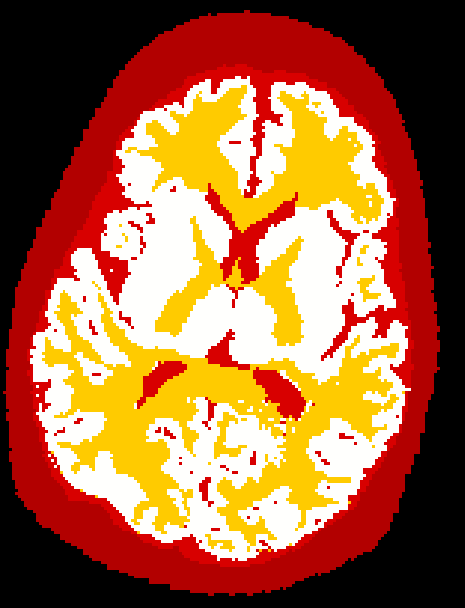
\includegraphics[height=3cm]{figures/simulation_input_pet.png}};

		\node[mybox, below=1.7cm of t1, minimum width=3cm] (simpet) {Simulated PET};
		\node[below=0.5cm of simpet] (phantom_image) {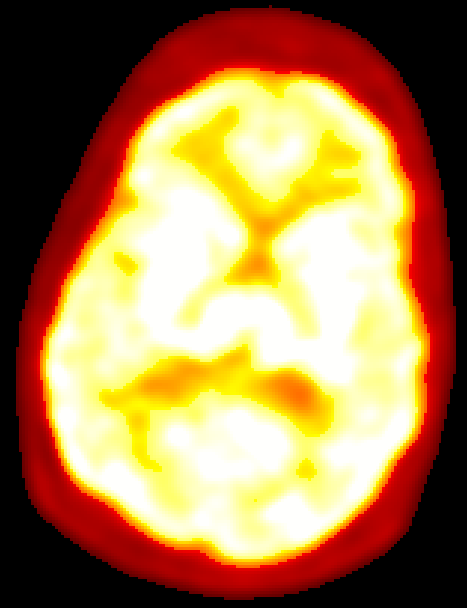
\includegraphics[height=3cm]{figures/simulated_pet.png}};

		\draw[->]
		(pet.east) to[out=0, in=180]
		node[yshift=+2pt, above] {\textit{Compartmental Fitting}}
		node[yshift=-2pt, below] {\textit{\& PVC}}
		(ttac.west);

		\draw[->]
		(t1.east) to[out=0, in=180]
		node[yshift=+2pt, above] {\textit{Tissue}}
		node[yshift=-2pt, below] {\textit{Classification}}
		(phantom.west);

		\draw[->] (ttac.east) to[out=0, in=0] (proto.east);

		\draw[->] (phantom.east) to[out=0, in=0] (proto.east);

		\draw[->]
		(proto.west) to[out=180, in=0]
		node[yshift=+2pt, above] {\textit{Monte Carlo}}
		node[yshift=-2pt, below] {\textit{Simulation}}
		(simpet.east);

		\begin{pgfonlayer}{background}
			\draw[dashed, rounded corners, thick]
			($(pet.north west)+(-0.3,0.3)$) rectangle ($(t1.south east)+(0.3,-0.3)$);
		\end{pgfonlayer}
		\node at ($(t1.south)-(0,0.5)$) {\text{Real Life Data}};

		\begin{pgfonlayer}{background}
			\draw[dashed, rounded corners, thick]
			($(ttac.north west)+(-0.3,0.3)$) rectangle ($(phantom.south east)+(0.3,-0.3)$);
		\end{pgfonlayer}
		\node at ($(phantom.south)-(0,0.5)$) {\text{Ground Truth}};
	\end{tikzpicture}
	\caption{Simulation pipeline linking real data, derived ground-truth inputs, and simulated PET output.}\label{fig:sim_pipeline}
\end{figure}
